\section{Introduction}

Cluster computing enables us to perform a huge amount of computations on big data and get insights from them at a scale that a single machine can hardly achieve.
However, developing parallel programs to take advantage of a large cluster can be very difficult.

\begin{figure}
  \begin{center}
  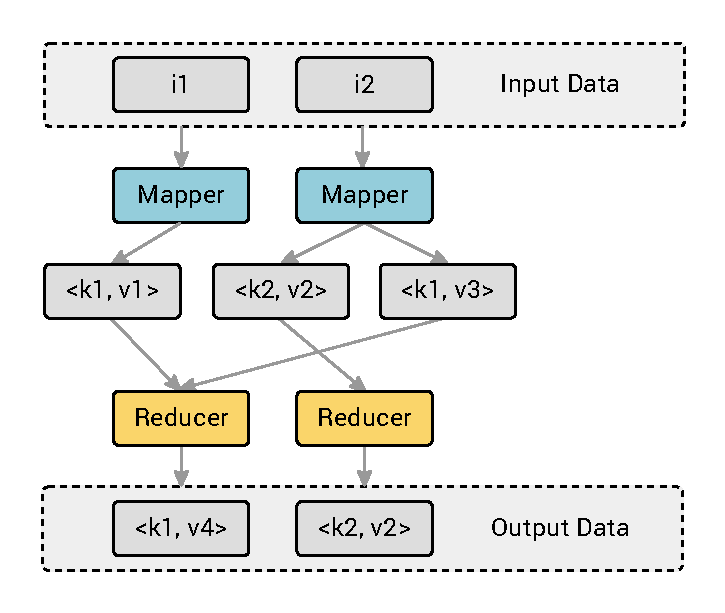
\includegraphics[width=\linewidth]{mr0.eps}
  \end{center}
  \vspace{-0.2cm}
  \caption{MapReduce Programming Model.
  The map function generates a set of intermediate key/value pairs for each input.
  The reduce function merges the values associated with the same key.
  Numerous data mining and machine learning algorithms are expressible with this model.
  }
  \label{fig:mr}
\end{figure}

MapReduce~\cite{dean2008mapreduce,dean2010mapreduce} greatly simplified this task by providing users a high-level abstraction for defining their computation, and taking care of the intricate low-level execution steps internally.
Fig.~\ref{fig:mr} illustrates the MapReduce programming model.
Logically, each MapReduce operation consists of two phases: a map phase where each input is mapped to a set of intermediate key/value pairs, and a reduce phase where the pairs with the same key are put together and reduced to a single key/value pair according to a user specified reduce function.


Many data mining algorithms are expressible with this model, such as PageRank~\cite{bahmani2011fast,plimpton2011mapreduce,ekanayake2010twister}, k-means~\cite{zhao2009parallel,chu2007map,cui2014optimized,anchalia2013mapreduce,ekanayake2008mapreduce,gopalani2015comparing}, Gaussian mixture model~\cite{chu2007map}, and k-nearest neighbors~\cite{anchalia2014k,maillo2015mapreduce,lu2012efficient,yokoyama2012processing}.

Although logically expressible, achieving similar efficiency as a hand-optimized parallel code is hard, especially when the data can be fit distributed into the memory.
In such cases, the file system is no longer the bottleneck and the overhead from MapReduce can make the execution much slower than hand-optimized code.

Google's MapReduce~\cite{dean2008mapreduce,dean2010mapreduce} and most of its variants~\cite{hadoop,chambers2010flumejava,cascading,afrati2010optimizing,bhatotia2011incoop,condie2010mapreduce,ekanayake2010twister,goiri2015approxhadoop,he2008mars,li2015coded,zaharia2008improving,yang2007map} save intermediate data and result to the file system even when the data can be fit into the memory.
Hence, its MapReduce performance is severely limited by the performance of the file system.

Spark~\cite{spark, zaharia2010spark, zaharia2016apache, zaharia2012resilient} offers an in-memory implementation of MapReduce, which is much faster than Google's MapReduce.
However, it uses a similar algorithm as Google's MapReduce, which is designed for disk-based data intensive use cases and does not consider the computational overheads of MapReduce seriously.
Hence, the performance of Spark is often far from the performance of hand-optimized code.

To achieve better performance while preserving the high-level MapReduce abstraction, we develop Blaze, a C++ based cluster computing library that focuses on in-memory high performance MapReduce and related operations.
Blaze introduces three main improvements to the MapReduce algorithm: eager reduction, fast serialization, and special treatment for a small fixed key range.
Section~\ref{sec:opt} provides a detailed description of these improvements.



% Blaze is  quantum chemistry package~\cite{li2018fast}.
% Blaze has already been used in a quantum chemistry package~\cite{li2018fast} to make the code more maintainable without sacrificing the performance.
% Together with that quantum chemistry package, Blaze has been run for tens of millions of core-hours by several top research groups to perform highly accurate quantum simulations and aid the discovery of new materials and new chemical processes.

% The highly-optimized in-memory MapReduce implementation can be very useful to numerous data mining and machine learning related tasks.

We apply Blaze to several common data mining tasks, including word frequency count, PageRank, k-means, expectation maximization (Gaussian mixture), and k-nearest neighbors.
Our results show that Blaze is on average 10 times faster than Spark on these tasks.
% We compare its performance with Apache Spark and results

The main contributions of this research are listed as follows:
\begin{enumerate}
    \item We develop Blaze, a high performance cluster computing library that allows users to write parallel programs with the high-level MapReduce abstraction while achieving similar performance as hand-optimized code for compute intensive tasks.
    \item We introduce three main performance improvements to the MapReduce algorithm to make it more efficient: eager reduction, fast serialization, and special treatment for a small fixed key range.
    \item We apply Blaze to 5 common data mining tasks and demonstrate that Blaze programs are easy to develop and can outperform Apache Spark programs by more than 10 times on average for these tasks.
    % by applying the improvements above, we can keep the simple high-level abstraction of MapReduce while achieving $10 \times$ higher performance than Apache Spark on some common data mining and machine learning tasks.
\end{enumerate}

The remaining sections are organized as follows:
Section~\ref{sec:blaze} describes the Blaze framework and the details of the optimization.
Section~\ref{sec:app} present the details of how we implement several key data mining and machine learning algorithms with Blaze and compare the performance with Apache Spark.
Section~\ref{sec:con} concludes the paper.

% {\color{gray}
% Blaze is originally designed for quantum chemistry to make the code more flexible and extensible while preserving the performance of low level hand optimized code, so that researchers can add new features and test new ideas faster.
% We find that most quantum chemistry methods can be implemented as a series of map and reduce operations, so we use the MapReduce paradigm to re-engineer our quantum chemistry package.
% We then carefully profile the code and introduce lots of optimizations to our MapReduce implementation to make the re-engineered code run even faster than the original hand-optimized code.
% Arrow is the code name for the re-engineered version.
% Although developed less than a year ago, Arrow is already being used in several top research groups.
% Tens of millions of core-hours of calculations have been performed with Arrow for various types of chemical systems and methods.
% In our largest calculation, we use our custom MapReduce to solve for the lowest few eigenvalues of a sparse Hamiltonian matrix of size $10^{29} \times 10^{29}$, where we repeatedly process of trillions of non-zero matrix elements deterministically and $10^{32}$ other non-zero matrix elements stochastically~\cite{li2018fast}.

% We find that the optimizations that we introduced to MapReduce can be useful to lots of data mining and related tasks as well, so we factor out our MapReduce implementation, together with some other utility functions and distributed data containers into a standalone library, and give it the name Blaze.
% }

% \section{Related Works}
% \label{sec:rel}
% Here we breifly review the previous MapReduce works in two directions: traditional MapReduce workflow and data mining oriented MapReduce workflow. 
% % We then discuss how Blaze could outperform prior MapReduce frameworks.

% \subsection{Traditional MapReduce Workflow}
% Original MapReduce~\cite{dean2008mapreduce,dean2010mapreduce} provides a high-level abstraction for computations that can be expressed as three simple steps 1) map, 2) shuffle, 3) and reduce, where both C++ and Java can be used to program the applications, as is shown in the upper panel of Fig.~\ref{fig:mrdiff}.
% This MapReduce framework is designed for data intensive workflows at Google and its algorithm is specially optimized for hard disk drives.
% % However, as most data mining and machine learning applications could be expressed with data streaming procedures, hard disk drives are no longer needed for data flows among these three steps. 

% Hadoop~\cite{hadoop} is an open-source implementation of MapReduce based on Java, together with some other utilities such as the Hadoop File System (HDFS).
% % Though Hadoop provides more user-friendly interface,
% Java-based Hadoop code can be slower than carefully programmed C++ based Google MapReduce code.
% However, the difference is often negligible because the bottleneck of both original MapReduce and Hadoop are the file system.
% % and their lack of performance optimization for data mining and machine leanrning applications. 

% FlumeJava~\cite{chambers2010flumejava} builds on Java MapReduce and offers a set of more primitive abstractions and an optimizer for achieving similar performance as hand-optimized MapReduce pipelines.
% As such, the performance of FlumeJava is still limited by the performance of the original Google MapReduce.
% Cascading~\cite{cascading} builds on Hadoop to provide better abstractions and optimizations and has similar performance as FlumeJava.

% Map-Reduce-Merge~\cite{yang2007map} adds a Merge phase to Map-Reduce to support processing multiple related heterogeneous datasets efficiently.
% However, the performance of Map-Reduce-Merge is still limited by the performance of the file system.
% % Therefore, it is imperative to have an efficient MapReduce implementation that could provide in-memory operations.

% \subsection{Data Mining Oriented Workflow} 
% Spark~\cite{spark, zaharia2010spark, zaharia2016apache, zaharia2012resilient} offers in-memory implementation of MapReduce, together with some other primitive parallel abstractions and high-level domain-specific parallelization libraries. 
% GraphX~\cite{xin2013graphx} and MLlib~\cite{meng2016mllib} are among the popular ones of them.
% Specifically, with in-memory excutable Spark, libraries such as MLlib~\cite{meng2016mllib} could be used more efficiently for certain data mining and machine learning related tasks.  
% Though Spark can run some workloads much faster than Hadoop~\cite{shi2015clash,gopalani2015comparing}, it sticks to the original MapReduce algorithm and does not provide efficient optimization for in-memory executions for data mining and machine learning applications.
% In addition, Spark is written in Scala, a programming language on Java, which introduces more computational overheads and higher memory footprints than C++.

% With Spark, numerous MapReduce adaptions for data mining and machine learning algorithms have been studied in lots of literatures~\cite{zhao2009parallel, ekanayake2008mapreduce, gopalani2015comparing, esmaeilpour2016distributed, lu2012efficient, stupar2010rankreduce, anchalia2014k, maillo2015mapreduce, eldawy2013demonstration, wang2010accelerating, song2015solutions}.
% For example, Chu et al.~\cite{chu2007map} implements a group of machine learning algorithms using the map-and-reduce style, including K-means and expectation maximizations (with Gaussian Mixture Model), and achieves almost linear speed up with the number of cores on a single machine.
% Matrix computations are important parts for many data mining and machine learning tasks, so Zadeh et al.~\cite{bosagh2016matrix} designs a matrix separating and shipping scheme for more efficient matrix computations based on Spark.
% However, these domain-specific implementations neither lack of efficient communications for distributed computations or only with a narrow application area. 
% Hence, it is important to develop an efficient and unified MapReduce framework for data mining and machine learning applications.  


% \subsection{Blaze: Optimized MapReduce for Data Mining}

% Prior MapReduce works cannot fit well into modern data mining applications as described above. 
% However, Blaze targets high performance in-memory computations with C++, which performs memory-only computations during both shuffle and reduce phases.
% With its algorithm optimized for in-memory executions, it achieves much higher performance compared to original MapReduce when fitting the working data to the whole memory of the cluster.
% These optimized in-memory operations could achieve similar effects as hand-optimized parallel code based on low-level operations.
% % When the input data has to be read from the filesystem, the performance of Blaze will still be faster than MapReduce because of the four optimizations that we introduced in Blaze.

% In addition, the interface of Blaze makes developing parallel program similar to developing a serial program, which is more user-friendly than original MapReduce and Hadoop.
% Equipped with these advantageous properties, Blaze could easily outperform FlumeJava and improved Cascading framework.
% Blaze MapReduce also allows using mutable distributed data containers as the target container which naturally supports merge operations.
% With pure in-memory MapReduce implementation in Blaze, the file system is no long the bottleneck, Blaze is on average an order of magnitude faster than Spark on most common data mining tasks.
% Thanks to the various merits of Blaze framework, we could easily extend this work to multiple machines with multiple cores and still achieves linear speedup.
% All these advantages make Blaze a nice MapReduce framework for general data mining and machine learning tasks.
% Well will discuss later in details of the Blaze properties.
% % Some researchers pointed out that plenty of iterative algorithms, such as k-means, do not work well with the origin MapReduce and proposed various solutions to solve this problem~\cite{cui2014optimized,ekanayake2008mapreduce}.
% % Blaze works well for iterative algorithms and thus does not need any special modifications for these algorithms.